% Type of the document
\documentclass{beamer}

% elementary packages:
\usepackage{graphicx}
\usepackage[latin1]{inputenc}
\usepackage[T1]{fontenc}
\usepackage[english]{babel}
\usepackage{listings}
\usepackage{xcolor}
\usepackage{eso-pic}
\usepackage{mathrsfs}
\usepackage{url}
\usepackage{amssymb}
\usepackage{amsmath}
\usepackage{multirow}
\usepackage{hyperref}
\usepackage{booktabs}
\usepackage{tikz}

% additional packages
\usepackage{bbm}

% packages supplied with ise-beamer:
\usepackage{cooltooltips}
\usepackage{colordef}
\usepackage{beamerdefs}
\usepackage{lvblisting}

% Change the pictures here:
% logobig and logosmall are the internal names for the pictures: do not modify them. 
% Pictures must be supplied as JPEG, PNG or, to be preferred, PDF
\pgfdeclareimage[height=2cm]{logobig}{hulogo}
% Supply the correct logo for your class and change the file name to "logo". The logo will appear in the lower
% right corner:
\pgfdeclareimage[height=0.7cm]{logosmall}{Figures/LOB_Logo}

% Title page outline:
% use this number to modify the scaling of the headline on title page
\renewcommand{\titlescale}{1.0}
% the title page has two columns, the following two values determine the percentage each one should get
\renewcommand{\titlescale}{1.0}
\renewcommand{\leftcol}{0.6}

% Define the title.Don't forget to insert an abbreviation instead 
% of "title for footer". It will appear in the lower left corner:
\title[Short Title - please modify the figure in the lower right corner:]{The title of the talk can even be much longer than this}
% Define the authors:
\authora{Uwe Ziegenhagen} % a-c
\authorb{Stephan Stahlschmidt}
\authorc{}

% Define any internet addresses, if you want to display them on the title page:
\def\linka{http://lvb.wiwi.hu-berlin.de}
\def\linkb{}
\def\linkc{}
% Define the institute:
\institute{Ladislaus von Bortkiewicz Chair of Statistics \\
Humboldt--Universit�t zu Berlin \\}

% Comment the following command, if you don't want, that the pdf file starts in full screen mode:
\hypersetup{pdfpagemode=FullScreen}

%Start of the document
\begin{document}

% create the title slide, layout controlled in beamerdefs.sty and the foregoing specifications
\frame[plain]{
\titlepage
}

% The titles of the different sections of you talk, can be included via the \section command. The title will be displayed in the upper left corner. To indicate a new section, repeat the \section command with, of course, another section title
%%%%%%%%%%%%%%%%%%%%%%%%%%%%%%%%%%%%%%%%%%%%%%%%%%%%%%%%%%%%%%%%%%%%%%%%%%%%%%%%%%%%%%%%%%%%%%%%%%%%%%%%%%%%%%%%%%%%%%%%
\section{Introduction}
%%%%%%%%%%%%%%%%%%%%%%%%%%%%%%%%%%%%%%%%%%%%%%%%%%%%%%%%%%%%%%%%%%%%%%%%%%%%%%%%%%%%%%%%%%%%%%%%%%%%%%%%%%%%%%%%%%%%%%%%

% (A numbering of the slides can be useful for corrections, especially if you are
% dealing with large tex-files)
%%%%%%%%%%%%%%%%%%%%%%%%%%%%%%%%%%%%%%%%%%%%%%%%%%%%%%%%%%%%%%%%%%%%%%%%%%%%%%%%%%%%%%%%%%%%%%%%%%%%%%%%%%%%%%%%%%%%%%%%
\frame{
\frametitle{Basics}
Statistics is understanding data by modelling it.

Data \( Y^{(n)} = (Y_{1},\ldots,Y_{n}) \) usually \emph{random}.

\( \mathbbm{P} = \mathscr{L}(Y^{(n)}) \), the \emph{unknown} joint distribution.

Statistical problem: to infer on \( \mathbbm{P} \) from the data \( Y^{(n)} \).

\emph{Parametric} modelling:
\begin{eqnarray*}
\mathbbm{P} = \mathbbm{P}_{\boldsymbol{\theta}} \in \left\{\mathbbm{P}_{\boldsymbol{\theta}}, \boldsymbol{\theta} \in \Theta \subset \mathbbm{R}^{p}\right\}.
\end{eqnarray*}

\emph{Nonparametric} modelling:
the parametric assumption is not fulfilled, or, equivalently,
\( p = \infty \).
}


%%%%%%%%%%%%%%%%%%%%%%%%%%%%%%%%%%%%%%%%%%%%%%%%%%%%%%%%%%%%%%%%%%%%%%%%%%%%%%%%%%%%%%%%%%%%%%%%%%%%%%%%%%%%%%%%%%%%%%%%
% No number on outline slide
\section{}
\useheadtemplate{%
    \raisebox{-0.75cm}{\parbox{\textwidth}{%
            \footnotesize{\color{isegray}%
                \insertsection\ \leavevmode\leaders\hrule height3.2pt depth-2.8pt\hfill\kern0pt\ }}}
}

\frame{
\frametitle{Outline}

\begin{enumerate}
\item Attract the audience \quad \checkmark
\item The scientific message
\item Explain the method
\item Simulations \& discussion of your results
\item Applications and examples
\item Almost EOT = end of talk
\item Provoke few questions
\item Audience: enjoy what you have learnt
\end{enumerate}
}

% No number on outline slide
\useheadtemplate{%
    \raisebox{-0.75cm}{\parbox{\textwidth}{%
            \footnotesize{\color{isegray}%
                \insertsection\ \leavevmode\leaders\hrule height3.2pt depth-2.8pt\hfill\kern0pt\ \thesection-\thepage}}}}
\setcounter{section}{1}

%%%%%%%%%%%%%%%%%%%%%%%%%%%%%%%%%%%%%%%%%%%%%%%%%%%%%%%%%%%%%%%%%%%%%%%%%%%%%%%%%%%%%%%%%%%%%%%%%%%%%%%%%%%%%%%%%%%%%%%%
\section{LvB Beamer Style}
%%%%%%%%%%%%%%%%%%%%%%%%%%%%%%%%%%%%%%%%%%%%%%%%%%%%%%%%%%%%%%%%%%%%%%%%%%%%%%%%%%%%%%%%%%%%%%%%%%%%%%%%%%%%%%%%%%%%%%%%

% Subsections are not visible on the actual slide, but are displayed as bookmarks in the pdf file. Their application facilitates an easy navigation trough large pdf files.
%%%%%%%%%%%%%%%%%%%%%%%%%%%%%%%%%%%%%%%%%%%%%%%%%%%%%%%%%%%%%%%%%%%%%%%%%%%%%%%%%%%%%%%%%%%%%%%%%%%%%%%%%%%%%%%%%%%%%%%%
\subsection{General ideas}
%%%%%%%%%%%%%%%%%%%%%%%%%%%%%%%%%%%%%%%%%%%%%%%%%%%%%%%%%%%%%%%%%%%%%%%%%%%%%%%%%%%%%%%%%%%%%%%%%%%%%%%%%%%%%%%%%%%%%%%%

%%%%%%%%%%%%%%%%%%%%%%%%%%%%%%%%%%%%%%%%%%%%%%%%%%%%%%%%%%%%%%%%%%%%%%%%%%%%%%%%%%%%%%%%%%%%%%%%%%%%%%%%%%%%%%%%%%%%%%%%
\frame{
\frametitle{The \texttt{Beamer}-Package}

\begin{itemize}
\item \texttt{Beamer} is the latest package to create slides with \LaTeX
\item Slides need to be compiled to PDF, not DVI/Postscript
\item Remember: PDFLaTeX accepts PNG, JPEG and PDF not EPS/PS
\item If you \emph{need} Postscript, RTFM
\end{itemize}
}

%%%%%%%%%%%%%%%%%%%%%%%%%%%%%%%%%%%%%%%%%%%%%%%%%%%%%%%%%%%%%%%%%%%%%%%%%%%%%%%%%%%%%%%%%%%%%%%%%%%%%%%%%%%%%%%%%%%%%%%%
\frame[containsverbatim]{
\frametitle{The LvB Beamer Style}

\begin{itemize}
\item The LvB Beamer Style is defined via \textit{beamerdefs.sty}, \textit{colordef.sty} and \textit{lvblisting.sty}, which must always be provided in the source folder.
\item All operators are to be defined by \verb(\operatorname{}(. Note the difference:\\
\begin{center}
\begin{tabular}{ll}
$\operatorname{Var}$ & defined by operatorname\\
$Var$ & not defined by operatorname
\end{tabular}
\end{center}
\item Remember to start and end the displaymath environment by \verb(\[( and \verb(\]( and not \verb($$(.
\end{itemize}
}

%%%%%%%%%%%%%%%%%%%%%%%%%%%%%%%%%%%%%%%%%%%%%%%%%%%%%%%%%%%%%%%%%%%%%%%%%%%%%%%%%%%%%%%%%%%%%%%%%%%%%%%%%%%%%%%%%%%%%%%%
\frame[containsverbatim]{
\frametitle{Predefined comands}

\begin{itemize}
\item For your convenience you may set up new commands via \verb(\newcommand{}{}(.
\item This has been done in the two following cases:
	\begin{itemize}
	\item Use \verb(\quantnet( to include the quantnet icon (right-aligned):\\
	\begin{center}
	\quantnet MVAboxcity
	\end{center}
	The name of the quantnet is to be written in black.
	\item Use \verb(\BBI{}( to link to the BBI:\\
	\begin{center}
	\BBI{Carl Friedrich Gauss}
	\end{center}
	\end{itemize}
\item Some commands are already defined, e.g. \verb(\ln( and \verb(\log(
\end{itemize}
}

%%%%%%%%%%%%%%%%%%%%%%%%%%%%%%%%%%%%%%%%%%%%%%%%%%%%%%%%%%%%%%%%%%%%%%%%%%%%%%%%%%%%%%%%%%%%%%%%%%%%%%%%%%%%%%%%%%%%%%%%
\frame[containsverbatim]{
\frametitle{Equations}
\begin{itemize}
\item Equations covering several lines may be written in the \textit{align} environment instead of the older \textit{eqnarray} environment.\\Only this way it can be ensured, that the colour of the equation and of the according equation numbering match.
\item \verb(align*( omits the equation numbering, as does \verb(\notag(.
\end{itemize}
\begin{columns}[onlytextwidth]
\begin{column}{0.5\textwidth}
	\begin{lstlisting}
	\begin{align}
	4x + 8 &= (3-2)^2\\
	4x &= -7 \notag \\
	x &= -\frac{7}{4}
	\end{align}
	\end{lstlisting}
\end{column}
\begin{column}{0.5\textwidth}
	\begin{align}
	\hspace{-1cm}4x + 8 &= (3-2)^2\\
	4x &= -7 \notag \\
	x &= -\frac{7}{4}
	\end{align}
\end{column}
\end{columns}
}

%%%%%%%%%%%%%%%%%%%%%%%%%%%%%%%%%%%%%%%%%%%%%%%%%%%%%%%%%%%%%%%%%%%%%%%%%%%%%%%%%%%%%%%%%%%%%%%%%%%%%%%%%%%%%%%%%%%%%%%%
\frame{
\frametitle{Tables}
\vspace{-0.5cm}
\begin{table}
\begin{center}
\begin{tabular}{cc} 
\hline\hline
Title & Title\\ 
\hline
2.13 & 1.45 \\
3.14 & 6.85 \\
\hline\hline
\end{tabular}
\caption{Include a short, but meaningful caption.}
\end{center}
\end{table}
\begin{itemize}
\item Follow the Cambridge University Press Style.
\item Not more than 2 decimal digits in a column.
\item Tables and their captions are to be written in black.
\end{itemize}
}

%%%%%%%%%%%%%%%%%%%%%%%%%%%%%%%%%%%%%%%%%%%%%%%%%%%%%%%%%%%%%%%%%%%%%%%%%%%%%%%%%%%%%%%%%%%%%%%%%%%%%%%%%%%%%%%%%%%%%%%%
\frame[containsverbatim]{
\frametitle{Tables}
\begin{lstlisting}
\begin{table}
\begin{center}
\begin{tabular}{cc} 
\hline\hline
Title & Title\\ 
\hline
2.13 & 1.45 \\
3.14 & 6.85 \\
\hline\hline
\end{tabular}
\caption{Include a short, but meaningful caption.}
\end{center}
\end{table}
\end{lstlisting}
}

%%%%%%%%%%%%%%%%%%%%%%%%%%%%%%%%%%%%%%%%%%%%%%%%%%%%%%%%%%%%%%%%%%%%%%%%%%%%%%%%%%%%%%%%%%%%%%%%%%%%%%%%%%%%%%%%%%%%%%%%
\frame[containsverbatim]{
\vspace*{-0.2cm}
\frametitle{Figures}
\begin{columns}
\begin{column}{0.45\textwidth}
\begin{lstlisting}
\begin{figure}[htb]
	\begin{center}
	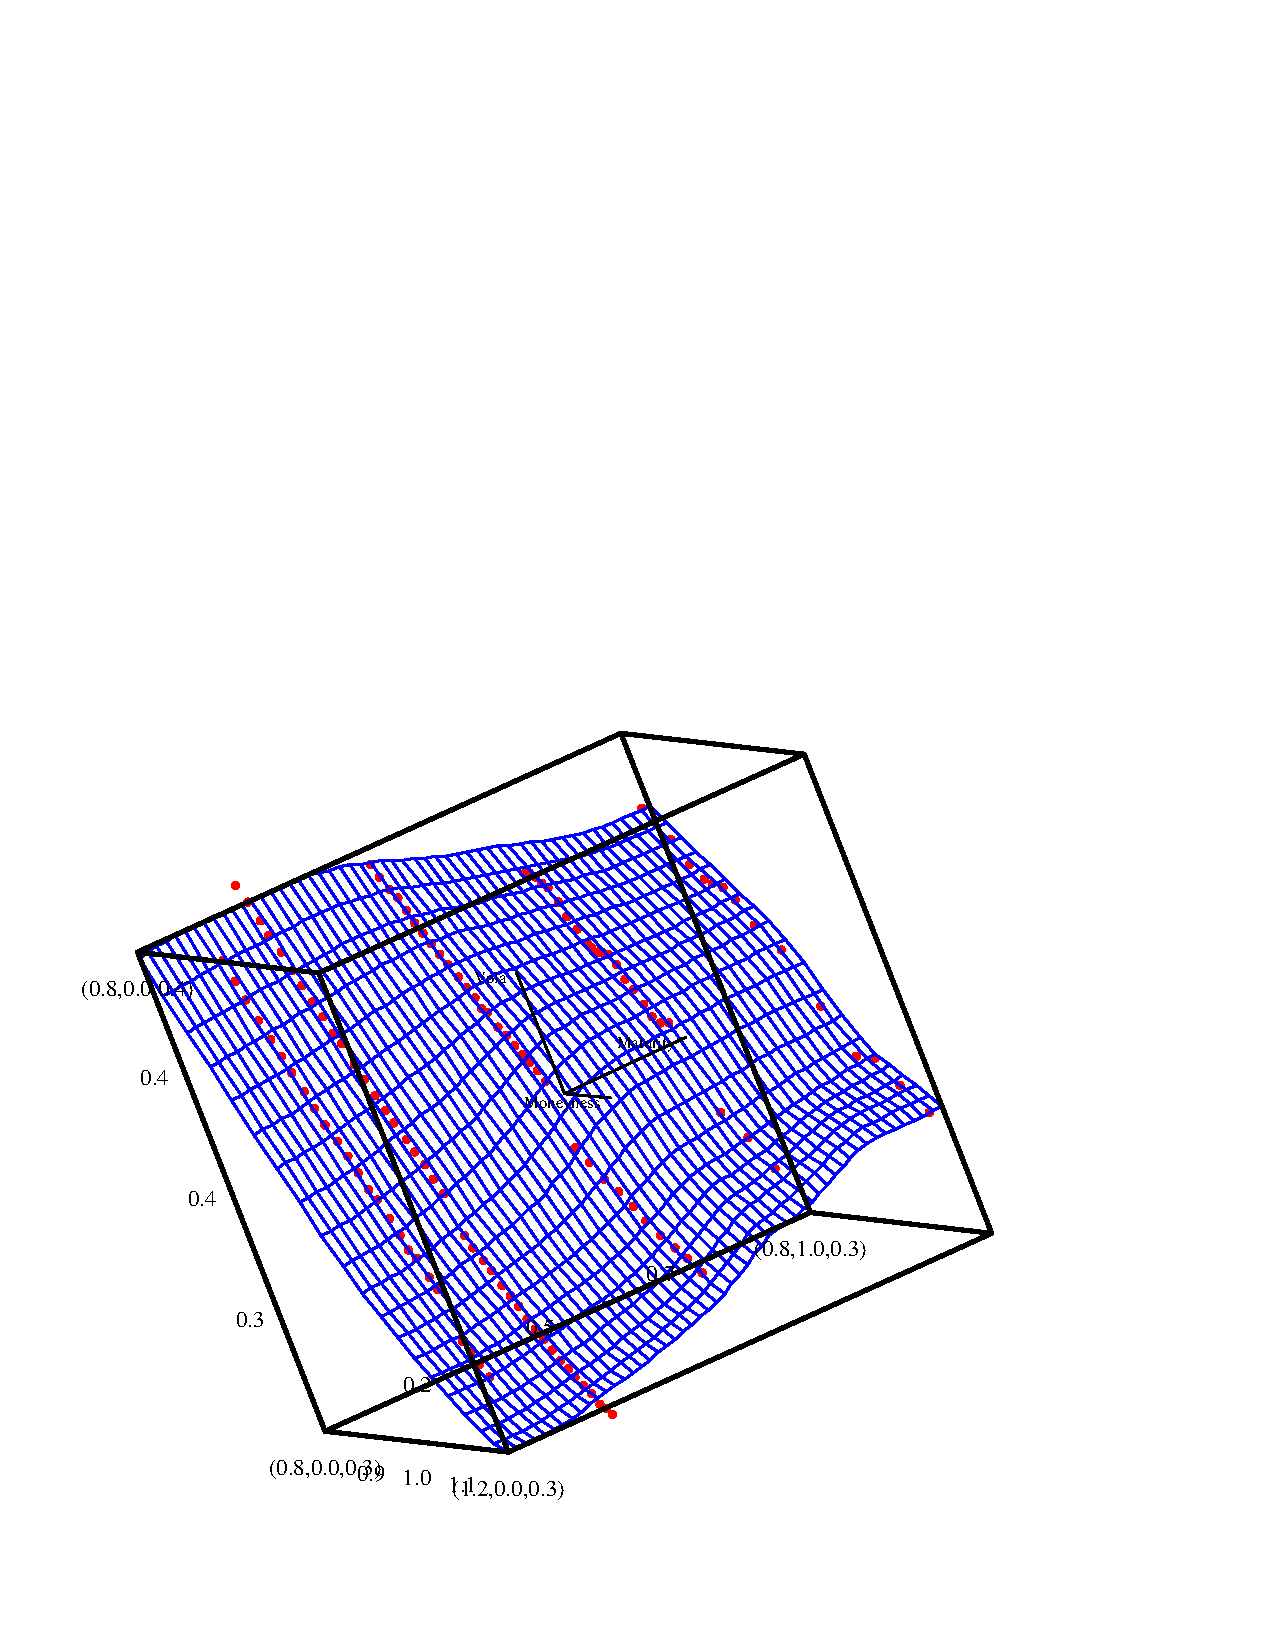
\includegraphics[scale=0.2]{Figures/vola}
	\caption{Include a short, but meaningful caption.}
	\end{center}
\end{figure}
\end{lstlisting}
\end{column}
\begin{column}{0.5\textwidth}
\begin{figure}[ht]
	\begin{center}
	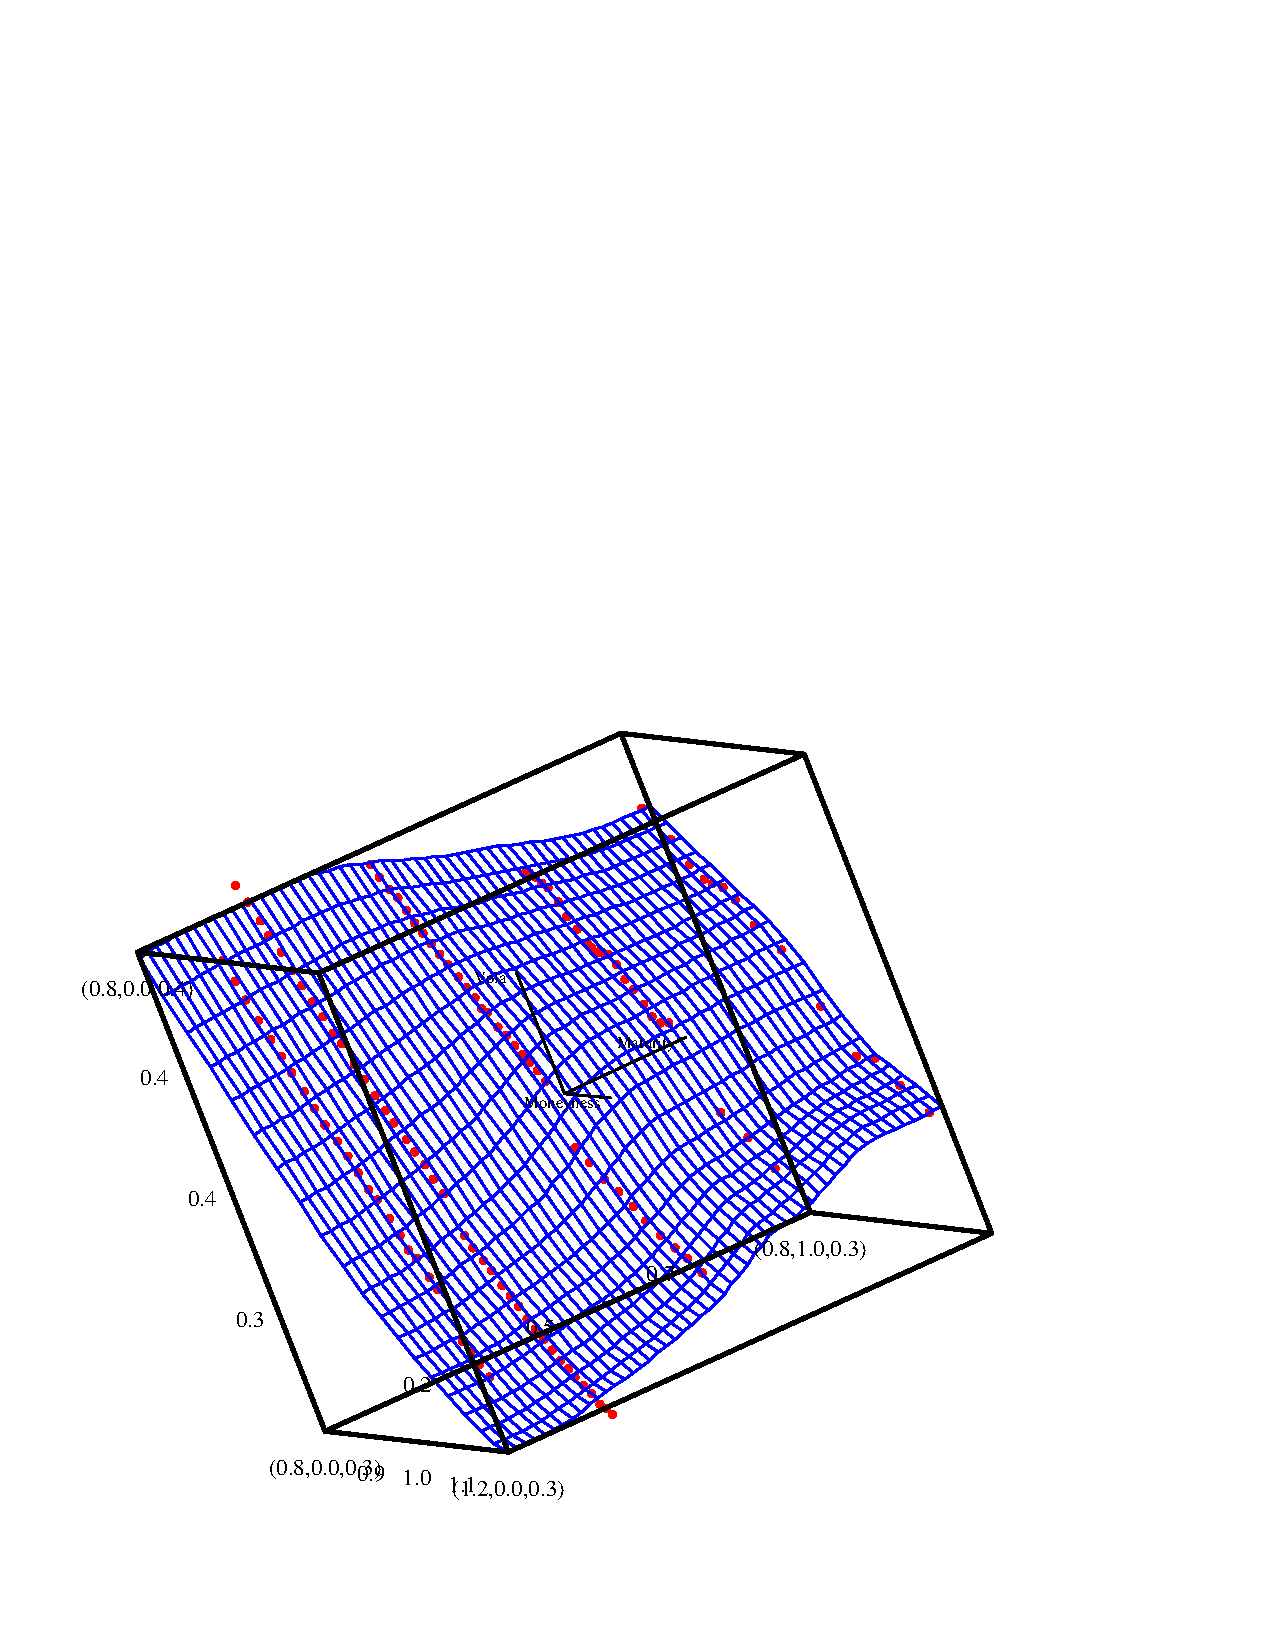
\includegraphics[scale=0.2]{Figures/vola}
	\caption{Include a short, but meaningful caption.}
	\end{center}
\end{figure}
\end{column}
\end{columns}
\vspace{0.2cm}
The caption is, as in tables, to be written in black and please provide any legend in the caption and not in the graph itself.
}

%%%%%%%%%%%%%%%%%%%%%%%%%%%%%%%%%%%%%%%%%%%%%%%%%%%%%%%%%%%%%%%%%%%%%%%%%%%%%%%%%%%%%%%%%%%%%%%%%%%%%%%%%%%%%%%%%%%%%%%%
\frame[containsverbatim]{
\frametitle{Examples}

To create an example, use the color \texttt{isegreen} and the following structure:

\begin{columns}[onlytextwidth]
\begin{column}{0.5\textwidth}
\begin{lstlisting}
\color{isegreen}
\textbf{Example:} Example title

\smallskip
Here you can state your example, which may also include calculations.
\color{black}
\end{lstlisting}
\end{column}
\hspace*{0.3cm}\begin{column}{0.5\textwidth}
\color{isegreen}
\textbf{Example:} Example title

\smallskip
Here you can state your example, which may also include calculations.
\color{black}
\end{column}
\end{columns}
}

%%%%%%%%%%%%%%%%%%%%%%%%%%%%%%%%%%%%%%%%%%%%%%%%%%%%%%%%%%%%%%%%%%%%%%%%%%%%%%%%%%%%%%%%%%%%%%%%%%%%%%%%%%%%%%%%%%%%%%%%
\frame[containsverbatim]{
\frametitle{Subtitles}
Subtitles are to be highlighted via bold text and followed by a small skip afterwards (no colon):

\begin{columns}[onlytextwidth]
\begin{column}{0.5\textwidth}
\begin{lstlisting}
\textbf{Subtitle}

\smallskip
Here you can state the content according to the subtitle.
\end{lstlisting}
\end{column}
\hspace*{0.3cm}\begin{column}{0.5\textwidth}
\textbf{Subtitle}

\smallskip
Here you can state the content according to the subtitle.
\end{column}
\end{columns}

\bigskip
This may also be applied to state proofs, theorems etc.
}

%%%%%%%%%%%%%%%%%%%%%%%%%%%%%%%%%%%%%%%%%%%%%%%%%%%%%%%%%%%%%%%%%%%%%%%%%%%%%%%%%%%%%%%%%%%%%%%%%%%%%%%%%%%%%%%%%%%%%%%%
\frame[containsverbatim]{
\frametitle{Brackets}
\begin{itemize}
	\item Use the bracket sequence $\left[\left\{\left(a+b=c\right)\right\}\right]$
	\item Conventional bracket rules represent an exemption of this rule. For example:
\[Y\sim \operatorname{N}(\mu(X), \sigma(X))\]
	\item Let \LaTeX\,take care about the correct size by preceding the bracket by \verb(\left( and \verb(\right(.
\end{itemize}
}

%%%%%%%%%%%%%%%%%%%%%%%%%%%%%%%%%%%%%%%%%%%%%%%%%%%%%%%%%%%%%%%%%%%%%%%%%%%%%%%%%%%%%%%%%%%%%%%%%%%%%%%%%%%%%%%%%%%%%%%%
\subsection{Rules}
%%%%%%%%%%%%%%%%%%%%%%%%%%%%%%%%%%%%%%%%%%%%%%%%%%%%%%%%%%%%%%%%%%%%%%%%%%%%%%%%%%%%%%%%%%%%%%%%%%%%%%%%%%%%%%%%%%%%%%%%

%%%%%%%%%%%%%%%%%%%%%%%%%%%%%%%%%%%%%%%%%%%%%%%%%%%%%%%%%%%%%%%%%%%%%%%%%%%%%%%%%%%%%%%%%%%%%%%%%%%%%%%%%%%%%%%%%%%%%%%%
\frame[containsverbatim]{
\frametitle{Rules to write nice slides}

\begin{itemize}
\item Use \verb(\section{}( and \verb(\subsection{}( to structure your presentation. The section will appear in the upper right corner of your slides.
\item You can set up hyperlinks via \verb(\label{LINKNAME}( (reference point) and \verb(\ref{LINKNAME}( (reference).
\item Use, if necessary, \verb(\displaystyle( to force \LaTeX to display fractions in big font size
\item Remember 
	\begin{itemize}
		\item 6-8 lines per slide
		\item 8 words per line
	\end{itemize}
\end{itemize}
}

%%%%%%%%%%%%%%%%%%%%%%%%%%%%%%%%%%%%%%%%%%%%%%%%%%%%%%%%%%%%%%%%%%%%%%%%%%%%%%%%%%%%%%%%%%%%%%%%%%%%%%%%%%%%%%%%%%%%%%%%
\frame[containsverbatim]{
\begin{itemize}
	\item The numbering of any enumeration should match the colour of the corresponding text (preset colour: black). Modifications may be made through the \textit{itemize} environment:
\begin{center}
\verb(\item[\color{isegreen}1.](
\end{center}
Itemize items are predefined (blue) and excluded from this rule.
	\item Use \verb(^{\top}( to write the symbol of transpose, it produces
\[ x^{\top}y \]
	\item Use \verb(\ldots( to write the symbol for three dots, it produces
\[ x \in \{1, \ldots, n \} \]
\end{itemize}
}

%%%%%%%%%%%%%%%%%%%%%%%%%%%%%%%%%%%%%%%%%%%%%%%%%%%%%%%%%%%%%%%%%%%%%%%%%%%%%%%%%%%%%%%%%%%%%%%%%%%%%%%%%%%%%%%%%%%%%%%%
\frame[containsverbatim]{
\begin{itemize}
	\item The commands \verb(\widehat{}( and \verb(\widetilde{}( for a hat or a tilde are to be preferred over the the smaller \verb(\hat( respectively \verb(\tilde( commands:\\
\begin{center}
$\widehat{Y}$ vs. $\hat{Y}$\\
$\widetilde{Y}$ vs. $\tilde{Y}$
\end{center}
	\item The norm is to be written via \verb(\|(. It produces $\|K\|$
	\item The $\mathcal{O}$ and {\scriptsize $\mathcal{O}$} for convergence may be written via \verb(\mathcal{O}( and \verb(\mbox{\scriptsize $\mathcal{O}$}(.
	\item The operator for exponential terms with Euler's $e$ as the base is defined by \verb(\exp(:
\[\exp(1) \approx 2.718282\]
\end{itemize}
}

%%%%%%%%%%%%%%%%%%%%%%%%%%%%%%%%%%%%%%%%%%%%%%%%%%%%%%%%%%%%%%%%%%%%%%%%%%%%%%%%%%%%%%%%%%%%%%%%%%%%%%%%%%%%%%%%%%%%%%%%
\frame[containsverbatim]{
\begin{itemize}
	\item Use \verb(\stackrel{\mathcal{L}}{\rightarrow}( to write the symbol for convergence in distribution and denote the normal distribution by \verb(\operatorname{N}(, this produces
\[ X \stackrel{\mathcal{L}}{\to} \operatorname{N}(0,\sigma^2) \]
	\item Use \verb(\operatorname{P}( to write the symbol for probability, it produces
\[ \operatorname{P} (X = x) = \frac{ \exp(- \lambda) {\lambda}^{x}}{{x}!} \]
	\item Use \verb(\stackrel{\operatorname{as.}}{\sim}( to write the symbol for asymptotic distribution, it produces \[ X \stackrel{\operatorname{as.}}{\sim} \chi^2\]
\end{itemize}
}

%%%%%%%%%%%%%%%%%%%%%%%%%%%%%%%%%%%%%%%%%%%%%%%%%%%%%%%%%%%%%%%%%%%%%%%%%%%%%%%%%%%%%%%%%%%%%%%%%%%%%%%%%%%%%%%%%%%%%%%%
\frame[containsverbatim]{
\begin{itemize}
	\item Use command \verb(\stackrel{\operatorname{def}}{=}( to write the symbol for definition, it produces \[ X \stackrel{\operatorname{def}}{=} \frac{a}{b} \] 
	\item Use commands \verb(\Re( or \verb(\Im( to write the symbols for the real or imaginary part, it produces \[ X = \Re \{Y \}, Y = \Im \{Z \} \]
	\item To write the symbols for the minimizing argument, use \verb(\operatorname{arg}\,\underset{x}{\operatorname{min}}(, it produces
\[ a = \operatorname{arg}\,\underset{x}{\operatorname{min}} \{f(x) \}\]
\end{itemize}
}

%%%%%%%%%%%%%%%%%%%%%%%%%%%%%%%%%%%%%%%%%%%%%%%%%%%%%%%%%%%%%%%%%%%%%%%%%%%%%%%%%%%%%%%%%%%%%%%%%%%%%%%%%%%%%%%%%%%%%%%%
\frame[containsverbatim]{
\begin{itemize}
	\item Use \verb(\operatorname{\mathbf{I}}( for the indicator function:
	\[ \operatorname{\mathbf{I}}\{x<1\}\]
	\item Use \verb(\log( to write the symbol for the natural logarithm, it produces
\[  1 = \log\{exp(1)\} \]
	\item Use \verb(\operatorname{E}( to write the symbol for expectation, it produces \[\operatorname{E}[X] = \mu \]
\end{itemize}
}

%%%%%%%%%%%%%%%%%%%%%%%%%%%%%%%%%%%%%%%%%%%%%%%%%%%%%%%%%%%%%%%%%%%%%%%%%%%%%%%%%%%%%%%%%%%%%%%%%%%%%%%%%%%%%%%%%%%%%%%%
\frame[containsverbatim]{
\begin{itemize}
    \item Use \verb(\hyperlink{labelname}{\beamerbutton{Link Name}}( to jump to other parts of your slides \\
    \hyperlink{labelname}{\beamerbutton{Link Name}}

\end{itemize}
}

%%%%%%%%%%%%%%%%%%%%%%%%%%%%%%%%%%%%%%%%%%%%%%%%%%%%%%%%%%%%%%%%%%%%%%%%%%%%%%%%%%%%%%%%%%%%%%%%%%%%%%%%%%%%%%%%%%%%%%%%
\subsection{Further topics}
%%%%%%%%%%%%%%%%%%%%%%%%%%%%%%%%%%%%%%%%%%%%%%%%%%%%%%%%%%%%%%%%%%%%%%%%%%%%%%%%%%%%%%%%%%%%%%%%%%%%%%%%%%%%%%%%%%%%%%%%

%%%%%%%%%%%%%%%%%%%%%%%%%%%%%%%%%%%%%%%%%%%%%%%%%%%%%%%%%%%%%%%%%%%%%%%%%%%%%%%%%%%%%%%%%%%%%%%%%%%%%%%%%%%%%%%%%%%%%%%%
\frame[containsverbatim]{
\label{labelname}
\frametitle{Using \texttt{listings} for source}

Slides containing a listing also need [containsverbatim] as option. For 'highlighting' of XploRe keywords see \texttt{listing.tex}.

\begin{center}
\begin{lstlisting}
library("metrics")                                   
randomize(10178)                                     
z=(uniform(n).>0.5)~(normal(n).<0.5)                
\end{lstlisting}
\end{center}
}

%%%%%%%%%%%%%%%%%%%%%%%%%%%%%%%%%%%%%%%%%%%%%%%%%%%%%%%%%%%%%%%%%%%%%%%%%%%%%%%%%%%%%%%%%%%%%%%%%%%%%%%%%%%%%%%%%%%%%%%%
\section{Piecewise Uncovering}
\subsection{Uncovering}
%%%%%%%%%%%%%%%%%%%%%%%%%%%%%%%%%%%%%%%%%%%%%%%%%%%%%%%%%%%%%%%%%%%%%%%%%%%%%%%%%%%%%%%%%%%%%%%%%%%%%%%%%%%%%%%%%%%%%%%%

%%%%%%%%%%%%%%%%%%%%%%%%%%%%%%%%%%%%%%%%%%%%%%%%%%%%%%%%%%%%%%%%%%%%%%%%%%%%%%%%%%%%%%%%%%%%%%%%%%%%%%%%%%%%%%%%%%%%%%%%
\frame{
\frametitle{Piecewise Uncovering I}

The following example uses $<1-2>$ commands to piecewise hide and uncover text. $<1-2>$ makes the first item appear only on slides 1 and 2, $<2->$ has the second item visible from slide 2 onwards.

\begin{itemize}
\item<1-2> Itemize environments
\item<2-> can be uncovered or hidden
\item<3-> piecewise.
\end{itemize}

\begin{enumerate}[<+->][(i)]
\item First Roman point.
\item Second Roman point, uncovered on second slide.
\item Last Roman point.
\end{enumerate}
}

%%%%%%%%%%%%%%%%%%%%%%%%%%%%%%%%%%%%%%%%%%%%%%%%%%%%%%%%%%%%%%%%%%%%%%%%%%%%%%%%%%%%%%%%%%%%%%%%%%%%%%%%%%%%%%%%%%%%%%%%
\frame{
\frametitle{Piecewise Uncovering II}

There is an easier way using $\mbox{\textbackslash item}<+->$

\begin{itemize}  
\item<+-> Itemize environments 
\item<+-> can be uncovered or hidden
\item<+-> piecewise.
\end{itemize}
}

%%%%%%%%%%%%%%%%%%%%%%%%%%%%%%%%%%%%%%%%%%%%%%%%%%%%%%%%%%%%%%%%%%%%%%%%%%%%%%%%%%%%%%%%%%%%%%%%%%%%%%%%%%%%%%%%%%%%%%%%
\subsection{Hidding}
%%%%%%%%%%%%%%%%%%%%%%%%%%%%%%%%%%%%%%%%%%%%%%%%%%%%%%%%%%%%%%%%%%%%%%%%%%%%%%%%%%%%%%%%%%%%%%%%%%%%%%%%%%%%%%%%%%%%%%%%

%%%%%%%%%%%%%%%%%%%%%%%%%%%%%%%%%%%%%%%%%%%%%%%%%%%%%%%%%%%%%%%%%%%%%%%%%%%%%%%%%%%%%%%%%%%%%%%%%%%%%%%%%%%%%%%%%%%%%%%%
\frame{
\frametitle{Hiding text\dots}

Text on the first slide.

\onslide<2-3>
Shown on second and third slide.

\begin{itemize}  
\item Still shown on 2nd and 3rd slide.
\onslide<4->
\item Shown from slide 4 on.
\onslide<3,5> 
\item Shown on slides 3 and 5. 
\end{itemize}
\onslide
Shown on all slides.
}

%%%%%%%%%%%%%%%%%%%%%%%%%%%%%%%%%%%%%%%%%%%%%%%%%%%%%%%%%%%%%%%%%%%%%%%%%%%%%%%%%%%%%%%%%%%%%%%%%%%%%%%%%%%%%%%%%%%%%%%%
\section{Further Information}
%%%%%%%%%%%%%%%%%%%%%%%%%%%%%%%%%%%%%%%%%%%%%%%%%%%%%%%%%%%%%%%%%%%%%%%%%%%%%%%%%%%%%%%%%%%%%%%%%%%%%%%%%%%%%%%%%%%%%%%%

%%%%%%%%%%%%%%%%%%%%%%%%%%%%%%%%%%%%%%%%%%%%%%%%%%%%%%%%%%%%%%%%%%%%%%%%%%%%%%%%%%%%%%%%%%%%%%%%%%%%%%%%%%%%%%%%%%%%%%%%
\frame{
\frametitle{Further Information}
Further Information can be found in the \LaTeX\, version of this document, where some more details are explained and important specifications are highlighted.

\bigskip
Suggestions to improve the style or the explanations are welcome!
}

%%%%%%%%%%%%%%%%%%%%%%%%%%%%%%%%%%%%%%%%%%%%%%%%%%%%%%%%%%%%%%%%%%%%%%%%%%%%%%%%%%%%%%%%%%%%%%%%%%%%%%%%%%%%%%%%%%%%%%%%
\frame{
\frametitle{For Further Reading}
\begin{thebibliography}{aaaaaaaaaaaaaaaaa}
\beamertemplatearticlebibitems
\bibitem{Oetiker:2006}
Tobias Oetiker, Hubert Partl, Irene Hyna and Elisabeth Schlegl
\newblock{\em The Not So Short Introduction to \LaTeX 2e}
\newblock available on \href{http://www.ctan.org/tex-archive/info/lshort/english/}{www.ctan.org}, 2008
\beamertemplatearticlebibitems
\bibitem{Pakin:2008}
Scott Pakin
\newblock{\em The Comprehensive \LaTeX Symbol List}
\newblock available on \href{http://www.ctan.org/tex-archive/info/symbols/comprehensive/}{www.ctan.org}, 2008
\beamertemplatebookbibitems
\bibitem{Eckel:2004}
Frank Mittelbach and Michel Goossens
\newblock {\em The \LaTeX{ }Companion -- 2nd ed.}
\newblock Addison-Wesley, 2004
\end{thebibliography}
}

%%%%%%%%%%%%%%%%%%%%%%%%%%%%%%%%%%%%%%%%%%%%%%%%%%%%%%%%%%%%%%%%%%%%%%%%%%%%%%%%%%%%%%%%%%%%%%%%%%%%%%%%%%%%%%%%%%%%%%%%
\frame{
\frametitle{For Further Reading}
\begin{thebibliography}{aaaaaaaaaaaaaaaaa}
\beamertemplatearticlebibitems
\bibitem{Trettin:2007}
Mark Trettin and J�rgen Fenn
\newblock{\em An essential guide to \LaTeX 2e usage}
\newblock available on \href{http://tug.ctan.org/cgi-bin/ctanPackageInformation.py?id=l2tabu-english}{www.ctan.org}, 2007
\beamertemplatearticlebibitems
\bibitem{wiki:index}
Wikipedia Wiki Books
\newblock{\em LaTeX-W�rterbuch: InDeX}
\newblock available on \href{http://de.wikibooks.org/}{www.wikipedia.de}
\beamertemplatearticlebibitems
\bibitem{Tantau:2007}
Till Tantau
\newblock{\em User Guide to the Beamer Class, Version 3.07}
\newblock available on \href{http://latex-beamer.sourceforge.net}{www.sourceforge.net}, 2007
\end{thebibliography}
}

% Define the end of the document:
\end{document}
